%%
%% This is file `sample-acmsmall.tex',
%% generated with the docstrip utility.
%%
%% The original source files were:
%%
%% samples.dtx  (with options: `acmsmall')
%% 
%% IMPORTANT NOTICE:
%% 
%% For the copyright see the source file.
%% 
%% Any modified versions of this file must be renamed
%% with new filenames distinct from sample-acmsmall.tex.
%% 
%% For distribution of the original source see the terms
%% for copying and modification in the file samples.dtx.
%% 
%% This generated file may be distributed as long as the
%% original source files, as listed above, are part of the
%% same distribution. (The sources need not necessarily be
%% in the same archive or directory.)
%%
%% Commands for TeXCount
%TC:macro \cite [option:text,text]
%TC:macro \citep [option:text,text]
%TC:macro \citet [option:text,text]
%TC:envir table 0 1
%TC:envir table* 0 1
%TC:envir tabular [ignore] word
%TC:envir displaymath 0 word
%TC:envir math 0 word
%TC:envir comment 0 0
%%
%%
%% The first command in your LaTeX source must be the \documentclass command.
\documentclass[sigplan]{acmart}
%% NOTE that a single column version is required for 
%% submission and peer review. This can be done by changing
%% the \doucmentclass[...]{acmart} in this template to 
%% \documentclass[manuscript,screen]{acmart}
%% 
%% To ensure 100% compatibility, please check the white list of
%% approved LaTeX packages to be used with the Master Article Template at
%% https://www.acm.org/publications/taps/whitelist-of-latex-packages 
%% before creating your document. The white list page provides 
%% information on how to submit additional LaTeX packages for 
%% review and adoption.
%% Fonts used in the template cannot be substituted; margin 
%% adjustments are not allowed.
%%
%% \BibTeX command to typeset BibTeX logo in the docs
\AtBeginDocument{%
  \providecommand\BibTeX{{%
    \normalfont B\kern-0.5em{\scshape i\kern-0.25em b}\kern-0.8em\TeX}}}

%% Rights management information.  This information is sent to you
%% when you complete the rights form.  These commands have SAMPLE
%% values in them; it is your responsibility as an author to replace
%% the commands and values with those provided to you when you
%% complete the rights form.
\setcopyright{acmcopyright}
\copyrightyear{2022}
\acmYear{2022}
\acmDOI{XXXXXXX.XXXXXXX}


%%
%% These commands are for a JOURNAL article.
\acmJournal{JACM}
\acmVolume{37}
\acmNumber{4}
\acmArticle{111}
\acmMonth{8}

%%
%% Submission ID.
%% Use this when submitting an article to a sponsored event. You'll
%% receive a unique submission ID from the organizers
%% of the event, and this ID should be used as the parameter to this command.
%%\acmSubmissionID{123-A56-BU3}

%%
%% The majority of ACM publications use numbered citations and
%% references.  The command \citestyle{authoryear} switches to the
%% "author year" style.
%%
%% If you are preparing content for an event
%% sponsored by ACM SIGGRAPH, you must use the "author year" style of
%% citations and references.
%% Uncommenting
%% the next command will enable that style.
%%\citestyle{acmauthoryear}

%%
%% Personal package imports
\usepackage{listings}
\usepackage{multirow}
\usepackage{dirtytalk}

% TODO: remove me
\usepackage{todonotes}
\setuptodonotes{inline}

%%
%% end of the preamble, start of the body of the document source.
\begin{document}

%%
%% The "title" command has an optional parameter,
%% allowing the author to define a "short title" to be used in page headers.
\title[Void Processes]{Void Processes: Minimising privilege by default on Linux}

%%
%% The "author" command and its associated commands are used to define
%% the authors and their affiliations.
%% Of note is the shared affiliation of the first two authors, and the
%% "authornote" and "authornotemark" commands
%% used to denote shared contribution to the research.
\author{Jake Hillion}
\affiliation{%
  \institution{University of Cambridge}
  \country{United Kingdom}
}
\email{jake.hillion@cl.cam.ac.uk}

%%
%% By default, the full list of authors will be used in the page
%% headers. Often, this list is too long, and will overlap
%% other information printed in the page headers. This command allows
%% the author to define a more concise list
%% of authors' names for this purpose.
%\renewcommand{\shortauthors}{Hillion}

%%
%% The abstract is a short summary of the work to be presented in the
%% article.
\begin{abstract}
Operating systems are providing more facilities for process isolation than ever before, realised in technologies such as Containers [CN] and systemd slices [CN]. These systems separate the design of the program from the systems that create privilege separation.
  
Void Processes take these techniques to the extreme, removing access to everything but syscalls from a process by default. This work focuses on adding back slivers of privilege to achieve functional applications with minimal privilege.
  
I present a summary of the privilege separation features in modern Linux, the system design of void processes, the language front-ends to support it, and an evaluation on a series of example applications. 
\end{abstract}

%%
%% The code below is generated by the tool at http://dl.acm.org/ccs.cfm.
%% Please copy and paste the code instead of the example below.
%%
\begin{CCSXML}
<ccs2012>
 <concept>
  <concept_id>10010520.10010553.10010562</concept_id>
  <concept_desc>Computer systems organization~Embedded systems</concept_desc>
  <concept_significance>500</concept_significance>
 </concept>
 <concept>
  <concept_id>10010520.10010575.10010755</concept_id>
  <concept_desc>Computer systems organization~Redundancy</concept_desc>
  <concept_significance>300</concept_significance>
 </concept>
 <concept>
  <concept_id>10010520.10010553.10010554</concept_id>
  <concept_desc>Computer systems organization~Robotics</concept_desc>
  <concept_significance>100</concept_significance>
 </concept>
 <concept>
  <concept_id>10003033.10003083.10003095</concept_id>
  <concept_desc>Networks~Network reliability</concept_desc>
  <concept_significance>100</concept_significance>
 </concept>
</ccs2012>
\end{CCSXML}

\ccsdesc[500]{Computer systems organization~Embedded systems}
\ccsdesc[300]{Computer systems organization~Redundancy}
\ccsdesc{Computer systems organization~Robotics}
\ccsdesc[100]{Networks~Network reliability}

%%
%% Keywords. The author(s) should pick words that accurately describe
%% the work being presented. Separate the keywords with commas.
\keywords{datasets, neural networks, gaze detection, text tagging}


%%
%% This command processes the author and affiliation and title
%% information and builds the first part of the formatted document.
\maketitle

\section{Introduction}

Void processes take advantage of modern Linux namespaces to attempt to run applications without exposing them to the system itself. Void processes use a mixture of Linux namespaces and file descriptive based capabilities to allow running purpose-built applications without expecting the support of the standard Linux system. During the process of building such a system, gaps in the kernel were exposed, given that this work is at the edge of what main spaces can achieve. This work will go onto detail the process of creating void processes themselves, re-adding features that these processes need to do useful work, and the learnings of what features are missing in the user-space kernel APIs to succeed in creating processes this way.

This work explores the question of what is an operating system by taking a novel approach to running applications with the system exposed in an entirely different way. Rather than limiting the access of a process or set of processes to the operating system, such as in containers, we instead limit the access to the operating system with more explicit methods per process. Interaction between processes is allowed by specifying such interaction statically at compile time, removing any separation between the application developer and the system controlling access to the application, unlike solutions such as SELinux.

\section{Motivation}
\label{sec:motivation}

This work aims to explore the limits of the Linux userspace APIs in the context of complete process isolation, producing a software ecosystem to support running applications with fully minimised privilege. Further, discussion will be made of which parts of the API are well-suited and which are not, and how they might be better designed. Finally, the performance of absolute separation is evaluated, to find out at what cost this can be achieved in the current kernel.

Void processes aim to serve a different purpose than containers. Rather than virtualising a different operating system with the same kernel, void processes aim to remove all but what is necessary to run the application from the current operating system. The cut down appearance of the OS is still the same OS, rather than bringing in new utilities and libraries from perhaps a different OS. It would be possible to include this feature as an extension, but it is not the primary goal. This difference is important when deciding the features of the application, particularly the decision to exclude time namespaces (§\ref{sec:time-namespaces}).

\subsection{Threat Model}
\label{section:threat-model}

I present a threat model in which application binaries are trusted absolutely. That is, the software provider had no ill intent, and once the binary is on disk, it will not change without permission. This means that one can trust the binary to set up its own security, as it is protecting not against malice by its own developers, but instead bugs in the software.

\todo{Finalise threat model}

\section{Background}

\subsection{Mount Namespaces}

Mount namespaces were by far the most challenging part of this project. When adding new features, they continuously raised problems in both API description, expected behaviour, and performance of the tools given. A comparison will be given in this section to two other namespaces, network and UTS, to show the significant differences in the design goals of mount namespaces. Much of the programming issue here comes from a fundamental lack of consistency between mount namespaces and other namespaces in Linux, which will be discussed further in this section.

\subsubsection{Copy-on-Write}

Comparing to network namespaces, a slightly more modern namespace [Table \ref{tab:namespaces}], we see a huge difference in what occurs when a new namespace is created. When creating a new network namespace, one is immediately placed into a void, a network namespace containing only a loopback adapter. That is, the process has no ability to interact with the outside network, and no immediate relation to the parent network namespace. To interact with alternate namespaces, one must explicitly create a connection between the two, or move a physical adapter into the new (empty) namespace. Mount namespaces, rather than creating a new and empty namespace, made the choice to create a copy of the parent namespace, in a copy-on-write fashion. That is, after creating a new mount namespace, the mount hierarchy appears much the same as before.

\subsubsection{Shared Subtrees}
\label{sec:shared-subtrees}

While some other namespaces are copy-on-write, for example UTS namespaces, they do not present the same problem as mount namespaces. Although UTS namespaces are copy-on-write, it is trivial to create a void by setting the hostname of the machine to a constant. This removes any relation to the parent namespace and to the outside machine. Mount namespaces instead maintain a shared pointer with most filesystems, more akin to not creating a new namespace than a copy-on-write namespace.

Shared subtrees \citep{pai_shared_2005} were introduced to provide a consistent view of the unified hierarchy between namespaces. Consider the example in Figure \ref{fig:shared-subtrees}. \texttt{unshare(1)} creates a non-shared tree, which presents the behaviour shown. Although \texttt{/mnt/cdrom} from the parent namespace has been bind mounted in the new namespace, the content of \texttt{/mnt/cdrom} is not the same. This is because the filesystem newly mounted on \texttt{/mnt/cdrom} is unavailable in the separate mount namespace. To combat this, shared subtrees were introduced. That is, as long as \texttt{/mnt/cdrom} resides on a shared subtree, the newly mounted filesystem will be available to a copy of \texttt{/mnt/cdrom} in another namespace.

\begin{figure*}
\begin{minipage}{.45\textwidth}

\begin{lstlisting}[frame=tlrb]{Name}
#
#
#
#
#
#
# mount /dev/sr0 /mnt/cdrom
# ls /mnt/cdrom
file_1 file_2
\end{lstlisting}

\end{minipage}\hfill
\begin{minipage}{.45\textwidth}

\begin{lstlisting}[frame=tlrb,showlines=true]{Name}
# unshare -m
# mount_container_root /tmp/a
# mount --bind \
    /mnt/cdrom /tmp/a/mnt/cdrom
# pivot_root /tmp/a /tmp/a/oldroot
# umount /tmp/a/oldroot
#
# ls /mnt/cdrom

\end{lstlisting}

\end{minipage}

\caption{Highly separated behaviour without shared subtrees between mount namespaces.}
\label{fig:shared-subtrees}
\end{figure*}

\texttt{systemd} made the choice to mount \texttt{/} as a shared subtree \citep{free_software_foundation_mount_namespaces7_2021}:

\say{Notwithstanding the fact that the default propagation type for new mount is in many cases \texttt{MS\_PRIVATE}, \texttt{MS\_SHARED} is typically more useful.  For this reason, \texttt{systemd(1)} automatically remounts all mounts as \texttt{MS\_SHARED} on system startup. Thus, on most modern systems, the default propagation type is in practice \texttt{MS\_SHARED}.}

This means that when creating a new namespace, mounts and unmounts are propagated in by default. Further, it means that mounts and unmounts are propagated out of the namespace. This can be highly confusing behaviour, and \texttt{unshare(1)} considers this behaviour inconsistent with the goals of unsharing - it immediately calls \texttt{mount("none", "/", NULL, MS\_REC|MS\_PRIVATE, NULL)} after \texttt{unshare(CLONE\_NEWNS)}. The reasoning for this is that containers created should not present the behaviour given in Figure \ref{fig:shared-subtrees}, and this behaviour is unavoidable unless the parent mounts are shared, while it is possible to disable the behaviour where necessary.

\subsubsection{Lazy unmounting}

Mount namespaces present further interesting behaviour when unmounting initial root filesystem. Although this may initially seem isolated to void processes, it is also a problem in a container type system. Consider again the container created in Figure \ref{fig:shared-subtrees} - the existing root must be unmounted after pivoting, to avoid keeping the container fully connected to the outside root.

Referring again to network namespaces, sockets continue to exist in their initial namespace, allowing for regular file-descriptor passing semantics \citep{biederman_re_2007}. Extending upon this socket behaviour is Wireguard, which creates adapters that may be freely moved between namespaces while continuing to connect externally from their initial parent \citep[§7.3]{donenfeld_wireguard_2017}.

Something which behaves differently is the memory mapping of a currently running process's binary. Considering the example in Listing \ref{lst:unshare-umount}, which shows a short C program and the result of running it, it is seen that the \texttt{/} mount is busy when attempting the unmount. Given that the process was created in the parent namespace, the behaviour of file descriptors would suggest that the process would maintain a link to the parent namespace for its own memory mapped regions. However, the fact that the otherwise empty namespace has a busy mount shows that this is not the case.

\lstset{caption={Behaviour when attempting to unmount / after an unshare.}}
\begin{lstlisting}[float,label={lst:unshare-umount}]
int main() {
	if (unshare(CLONE_NEWNS))
		perror("unshare");
	if (mount("none", "/", NULL,
	  MS_REC|MS_PRIVATE, NULL))
		perror("mount");
	if (umount("/"))
		perror("umount");
}
--
umount: Device or resource busy
\end{lstlisting}

A feature called lazy unmounting or \texttt{MNT\_DETACH} exists for situations where a busy mount still needs to be unmounted. Supplying the \texttt{MNT\_DETACH} flag to \texttt{umount2(2)} causes the mount to be immediately detached from the unified hierarchy, while remaining mounted until the last user has finished with it. While this initially seems like a good solution, this syscall is incredibly dangerous when combined with shared subtrees. This behaviour is shown in Figure \ref{fig:unshare-umount-lazy}, where a lazy (and hence recursive) unmount is combined with a shared subtree to disastrous effect.

\begin{figure*}
\begin{minipage}{.45\textwidth}

\lstset{caption={}}
\begin{lstlisting}[frame=tlrb,showlines=true]{Name}
# cat /proc/mounts | grep udev
udev /dev devtmpfs rw,nosuid,relati...
#
#
# cat /proc/mounts | grep udev
cat: /proc/mounts: No such file or...
\end{lstlisting}
\end{minipage}\hfill
\begin{minipage}{.45\textwidth}

\lstset{caption={}}
\begin{lstlisting}[frame=tlrb]{Name}
#
#
# unshare --propagation unchanged -m
# umount -l /
#
#
\end{lstlisting}

\end{minipage}

\caption{Behaviour when attempting to unmount / from an unshared shell with a shared mount.}
\label{fig:unshare-umount-lazy}
\end{figure*}

This behaviour raises questions about why a shared subtree, which exists as an object, would need to be detached recursively - decreasing the reference count to the shared subtree itself would seem sufficient. The inconsistency is best explained by looking at the development timeline for the three features here: mount namespaces, shared subtrees, and recursive lazy unmounts.

When lazy unmounting was added, in September 2001, the author said the following \citep{viro_patch_2001}:

\say{There are only two things to take care of -
	a) if we detach a parent we should do it for all children
	b) we should not mount anything on "floating" vfsmounts.
Both are obviously staisfied for current code (presence of children
means that vfsmount is busy and we can't mount on something that
doesn't exist).}

This logic held even in the presence of namespaces, with the intial patchset in February 2001 \citep{viro_patch_2001}, as mounts were not initially shared but duplicated between namespaces. However, when shared subtrees were added in January 2005 \citep{viro_rfc_2005}, this logic stopped holding.

When setting up a container environment, one calls \texttt{pivot\_root(2)} to replace the old root with a new root for the container. Then, the old root may be unmounted. Oftentimes the solution is to exec a binary in the new root first, meaning that the old root is no longer in use and may be unmounted. This works, as old root is only a reference in this namespace, and hence may be unmounted with children - the vfsmount in this namespace is not busy, in contradiction to the quotation.

If, instead, one wishes to continue running the existing binary, this is possible with lazy unmounting. However, the kernel only exposes a recursive lazy unmount. With shared subtrees, this results in destroying the parent tree. While this is avoidable by removing the shared propagation from the subtree before unmounting, the choice to have \texttt{MNT\_DETACH} aggressively cross shared subtrees can be highly confusing, and perhaps undersired behaviour in a world with shared subtrees.

\section{System Design}

\begin{figure}
    \centering
    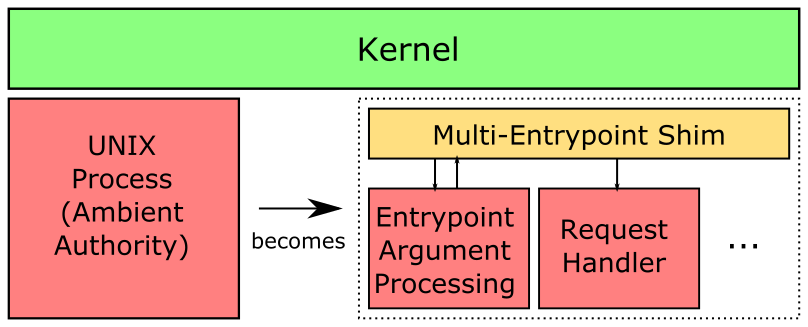
\includegraphics[width=\columnwidth]{figures/self-compartmentalisation-interactions.png}
    \caption{Interaction between the application and the environment.}
    \label{fig:self-compartmentalisation-interactions}
\end{figure}

An example of running a multi-entrypoint application is given in Figure \ref{fig:self-compartmentalisation-interactions}. What was originally a monolithic application becomes a set of applications that communicate with a new shim. The shim does not replace the kernel, and instead supplements it with new higher-level abilities. Each entrypoint receives input from the shim, and can return data to the shim where appropriate. Most of this data is in the form of file descriptors, which are treated as capabilities in this system.

A multi-entrypoint application stores the requirements for running it as static data in the ELF of the binary. When launched, \texttt{binfmt\_misc} is used to launch the application with the multi-entrypoint shim. The shim decodes this data and sets up processes and IPC accordingly.

The shim takes advantage of high levels of privilege to be able to more effectively deprivilege an application than an application with ambient authority could. For example, creating a new network namespace requires \texttt{CAP\_SYS\_ADMIN}, which would give many applications more privilege than they require. By deferring to a shim with extra privileges, this trusted code can be written only once, and avoid conferring more privileges than otherwise required.

\subsection{Building the Void}

Preparing a void for a new process takes advantage of the namespaces feature in Linux. However, many of the namespaces are not designed for this purpose, so this is a more difficult prospect than one might hope. Details of when each namespace was added and some of the relevant features are given in Table \ref{tab:namespaces}.

\begin{table*}
    \caption{Table showing the date and kernel version each namespace was added. The date provides the first commit where they appeared date of creation, and the kernel version the kernel release they appear in the changelog of. Namespaces are hence ordered by kernel version then alphabetically.}

    \begin{minipage}{\textwidth}
    \begin{center}
    \begin{tabular}{c|l|l|l}
        Namespace & CoW & Date & Kernel Version \\ \hline

        \texttt{mount}
            & $\boxtimes$ \footnote{Shared namespaces make for unique behaviour, see §\ref{sec:shared-subtrees}.}
            & 24th February 2001 \citep{viro_patchcft_2001}
            & 2.5.2 \citep{torvalds_linux_2002} \\
            
        \texttt{ipc}
            & $\square$
            & 2nd October 2006 \citep{korotaev_patch_2006}
            & 2.6.19 \citep{noauthor_linux_2006} \\

        \texttt{uts}
            & $\boxtimes$
            & 2nd October 2006 \citep{hallyn_patch_2006}
            & 2.6.19 \citep{noauthor_linux_2006} \\
            
        \texttt{user}
            & $\square$
            & 15th July 2007 \citep{le_goater_user_2007}
            & 2.6.23 \citep{noauthor_linux_2007} \\
            
        \texttt{network}
            & $\square$
            & 10th October 2007 \citep{biederman_net_2007}
            & 2.6.24 \citep{noauthor_linux_2008} \\
            
        \texttt{pid}
            & $\square$
            & 2nd October 2006 \citep{bhattiprolu_patch_2006}
            & 2.6.24 \citep{noauthor_linux_2008} \\
        
        \texttt{cgroup}
            & $\square$ \footnote{cgroup namespaces provide a virtualised view of the unified cgroup namespace and do not allow private modification.}
            & 18th March 2016 \citep{heo_git_2016}
            & 4.6 \citep{torvalds_linux_2016} \\

        \texttt{time}
            & $\boxtimes$
            & 12th November 2019 \citep{vagin_ns_2020}
            & 5.6 \citep{noauthor_linux_2020}

    \end{tabular}
    \end{center}
    \end{minipage}
    
    \label{tab:namespaces}
\end{table*}

\subsubsection{Mount namespaces}

Mount namespaces were the first [Table \ref{tab:namespaces}] namespaces introduced to Linux, in kernel version 2.5.2 [CN]. In contrast to network namespaces, the API is particularly unfriendly to creating a Void. The creation of mount namespaces is copy-on-write, and many filesystems are mounted shared. This means that they propagate changes back through namespace boundaries. As the mount namespace does not allow for creating an entirely new root, extra care must be taken in separating processes. The method taken in this system is mounting a new \texttt{tmpfs} file system in a new namespace, which doesn't propagate to the parent, and using the \texttt{pivot\_root(8)} command to make this the new root. By pivoting to the \texttt{tmpfs} without bind mounting the old root inside, the old root becomes completely inaccessible from the namespace. Similarly, the \texttt{tmpfs} never appears in the parent namespace. Finally, after ensuring the old root is set to \texttt{MNT\_PRIVATE} to avoid propagation (more details in §\ref{sec:shared-subtrees}), the old root can be lazily detached. This allows the binary from the parent namespace, the shim in this case, to continue running correctly. Any new processes only have access to the materials in the \texttt{tmpfs} void.

\subsubsection{ipc namespaces}

\todo{ipc namespaces}

\subsubsection{uts namespaces}

\todo{uts namespaces}

\subsubsection{user namespaces}

\todo{user namespaces}

\subsubsection{Network namespaces}

Network namespaces were added in kernel version 2.6.24 \citep{noauthor_linux_2008}, some time after the initial namespace boom. They present the optimal namespace for creating a void. Creating a new network namespace immediately creates an entirely empty namespace. That is, the new network namespace has no link whatsoever to the creating network namespace. To add a link, one can create a virtual Ethernet pair, with one adapter in each namespace [CN]. Alternatively, one can create a Wireguard adapter with sending and receiving sockets in one namespace and the VPN adapter in another \citep[§7.3]{donenfeld_wireguard_2017}. This allows for very high levels of separation while still maintaining access to the primary resource - the Internet or wider network.

\subsubsection{pid namespaces}

\todo{pid namespaces}

\subsubsection{cgroup namespaces}

\todo{cgroup namespaces}

\subsubsection{time namespaces}

Time namespaces are the final namespace added at the time of writing, added in kernel version 5.6 \citep{noauthor_linux_2020}. The motivation for adding time namespaces is given in the manual page [CN]:

\say{The  motivation  for adding time namespaces was to allow the monotonic and boot-time clocks to maintain consistent values during container migration and checkpoint/restore.}

That is, time namespaces virtualise the appearance of system uptime to processes, rather than attempting to virtualise the wall clock time.

\subsection{Filling the void}

Once a void has been created the goal is to reinsert enough to run the application, and no more. To allow for running applications in the void with minimal kernel changes, this is done using a mixture of file-descriptor capabilities and adding elements to the namespaces. Capabilities allow for a clean experience where suitable, while adding elements to namespaces creates a more Linux-like experience for the application.

\subsubsection{Files and directories} There are two options to provide access to files and directories in the void. Firstly, for a single file, an already open file descriptor can be offered. Consider the TLS broker of a TLS server with a persistent certificate and keyfile. Only these files are required to correctly run the application - no view of a filesystem is necessary. Providing an already opened file descriptor gives the process a capability to those files while requiring no concept of a filesystem, allowing that to remain a complete void. This is possible because of the semantics of file descriptor passing across namespaces - the file descriptor remains a capability, regardless of moving into a namespace without access to the file in question.

Alternatively, files and directories can be mounted in the void namespace. This supports three things which the capabilities do not: directories, dynamic linking, and applications which have not been adapted to use file descriptors. Firstly, the existing \texttt{openat(2)} calls are not suitable by default to treat directory file descriptors as capabilities, as they allow the search path to be absolute. This means that a process with a directory file descriptor in another namespace can access any files in that namespace [RN] by supplying an absolute path. Secondly, dynamic linking is best served by binding files, as these read only copies and the trusted binaries ensure that only the required libraries can be linked against. Finally, support for individual required files can be added by using file descriptors, but many applications will not trivially support it. Binding files allows for a final form of backwards compatibility.

\section{Language Frontends}

The language frontends are an extremely important part of this project, closing the gap between a static privilege separation solution like SELinux [CN] and a dynamic one like Capsicum \citep{watson_capsicum_2010}. I have implemented a language frontend in Rust and will describe it in this section.

\subsection{Rust}

\lstset{language=C,caption={A sample application using the Rust language frontend.}}
\begin{lstlisting}[float,label={lst:rust-language-frontend}]
#[entrypoint]
fn encrypt(mut in: File, mut out: File)

#[entrypoint]
fn main() {
  let input_file = ...;
  let output_file = ...;
  
  encrypt(input_file, output_file);
}
\end{lstlisting}

The Rust frontend uses macros to wrap functions with high-level primitives into multi-entrypoint compatible entrypoints. Further, it allows calling these functions using the new interface via the shim. Consider the example in Listing \ref{lst:rust-language-frontend}.

Firstly, the encrypt entrypoint is created. This is a regular Rust function which takes two high-level File objects, a wrapped file descriptor. The entrypoint macro wraps this function, providing in its place an \texttt{extern "C"} function that is unmangled and takes argc/argv. This allows functions with high-level arguments to be used as normal, with the argument parsing abstracted away by the library.

Second is the ordinary main function for the application. This is also tagged as an entrypoint, allowing the library to help out with more calls. The example given here is that of the encrypt method, which uses the API seen above. The use of macros here allows the call to encrypt to remain type safe, even though the call must pass through an external interface (the shim itself).

A significant benefit to this approach is the ease of disabling the multi-entrypoint application. By turning the entrypoint macro into identity with a crate feature, the code is compiled without the aid of the multi-entrypoint shim. This allows for significantly easier debugging, as the application follows a single execution path, rather than needing to be debugged as a distributed application.

\section{Example Applications}

\subsection{No Permissions}

The cornerstone of strong process separation is an application that is completely deprivileged. Listing \ref{lst:deprivileged-application} shows an application which, when run under the shim, drops all privileges except \texttt{stdout}. This is easy to achieve under the shim.

\lstset{language=C,caption={An application that requires only stdout and stderr.}}
\begin{lstlisting}[float,label={lst:deprivileged-application}]
#[entrypoint(stdout)]
fn main() { println!("hello world!"); }
\end{lstlisting}

\subsection{gzip}

GNU gzip \citep{gailly_gzip_2020} is well structured for privilege separation, though doesn't implement it by default. There is a clear split between the processing logic, selecting the items to do work on, and the compression/decompression routines, each of which are handed a pair of input and output file descriptors. This is shown by Watson et al. in \cite{watson_capsicum_2010}.

As C does not have high-level language features for multi-entrypoint applications, adapting it is slightly more verbose than the other examples seen. However, the resulting code change is still only X lines, if a bit more intricate. This places the risky compression and decompression routines in full sandboxes, while still allowing the simpler argument processing code ambient authority. The argument processing code needs no additional Linux capabilities to manage this permissioning, as the required capabilities are provided by the shim.

\subsection{TLS Server}

\begin{figure}
    \centering
    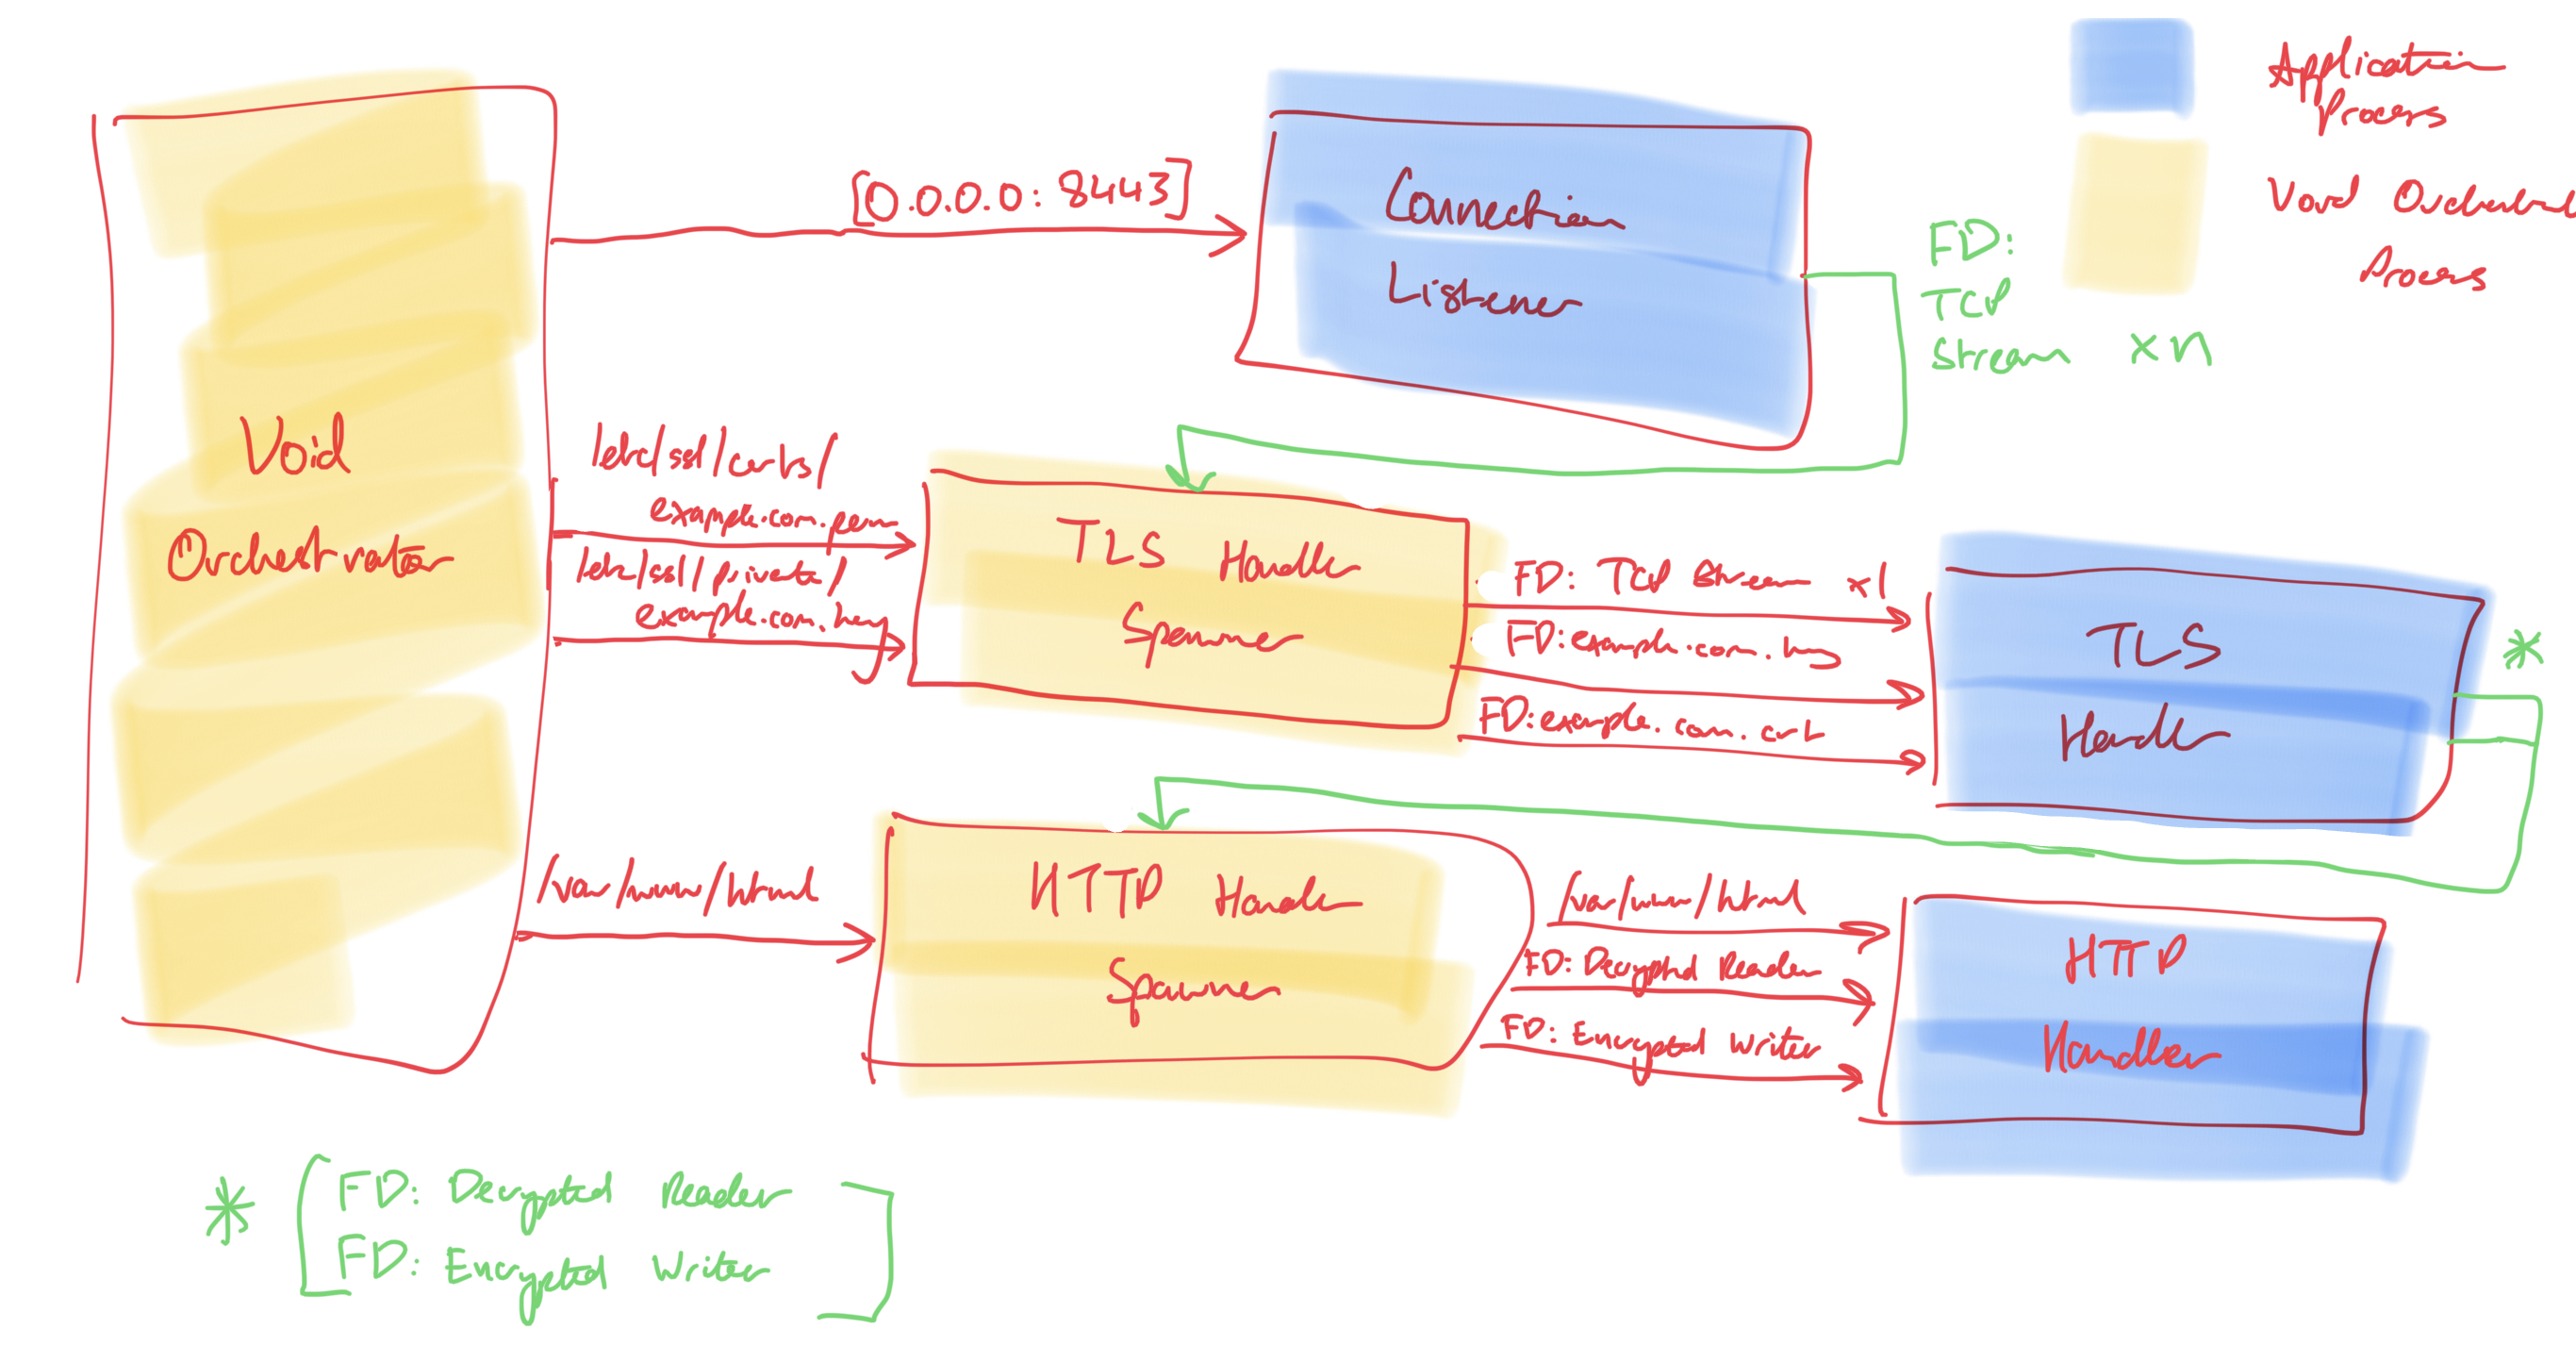
\includegraphics[width=\columnwidth]{figures/tls-server-splitting.png}
    \caption{Process separation in a TLS server.}
    \label{fig:tls-server-splitting}
\end{figure}

Finally, a rudimentary TLS server is created to show the rich privilege separation abilities of multi-entrypoint applications. An example structure is shown in Figure \ref{fig:tls-server-splitting}. Rather than being provided with a view of the network, the initial TCP handling process is given an already bound socket listener by the shim. This allows the TCP handler to live in an extremely restricted zero-access network namespace, while still performing the tasks of receiving new TCP connections.

Next, the TCP handler hands off the new TCP connections to the shim. Though the figure shows this as a direct connection between the TCP handler and the TLS handler, they are passed through the shim, from which the shim spawns a fresh TLS handler for each connection. The TLS handler is handed file descriptors to the certificate and key files that it requires, and hands back a decrypted request reader and an empty response writer file descriptor to the shim.

Finally, this pair of decrypted request reader and response writer are handed to a new process which handles the request. In the example case, this new process is handed a dirfd to \texttt{/var/www/html}, which is bind-mounted into an empty file system namespace by the shim. This allows the request handler enough access to serve files, while restricting access to anything else.

\section{Evaluation}

\todo{Write evaluation}

\section{Related Work}

\subsection{Virtual Machines and Containers}

Virtual Machine solutions \citep{barham_xen_2003,vmware_inc_understanding_2008} provide the ability to split a single machine into multiple virtual machines. When placing a single application in each virtual machine, they are effectively isolated from one another. Full fat container solutions such as Docker [CN], containerd [CN], and systemd-nspawn [CN] provide mechanisms to isolate an application almost completely from other applications running on a single machine. Some have claimed that this provides isolation superior to virtual machines \citep{soltesz_container-based_2007}.

Both of these solutions are less effective at isolating parts of an application from itself [CN with research]. Consider running only a TLS web server in a virtual machine. Although other applications will be unable to access the certificates, as they are in different virtual machines, methods within the application that should not be able to access the certificates still can.

While virtual machines and containers provide a strong isolation at the application level, they are not a compelling solution to intra-application privilege separation.

\subsection{systemd}

\texttt{systemd} [CN] provides a declarative interface to all of the process separation techniques used in this work. Rather than the responsibility of the programmer, creating these declarative descriptions is most commonly left to the package maintainers. This work seeks to provide similar capabilities to the people best suited to privilege separating an application: the developers.

\subsection{Capsicum}

Capsicum \citep{watson_capsicum_2010} extends UNIX file descriptors in FreeBSD to reflect the rights on the object they hold. These capabilities may be shared between processes as other file descriptors. The goals of both software are the same: make privilege separated software better. However, we take quite different approaches. Multi-entrypoint applications focus on building a static definition really close to the code, while Capsicum allows processes to dynamically privilege separate. This allows applying static analysis to the policies, while also keeping the definition close to the code.

\section{Future Work}

\subsection{Dynamic Linking}

Dynamic linking works correctly under the shim, however, it currently requires a high level of manual input. Given that the threat model in Section \ref{section:threat-model} specifies trusted binaries, it is feasible to add a pre-linking phase which mounts read-only libraries automatically in the environment for each spawned process.

\todo{Finish section on dynamic linking future work}

\section{Conclusion}

\todo{Write conclusion}

%%
%% The acknowledgments section is defined using the "acks" environment
%% (and NOT an unnumbered section). This ensures the proper
%% identification of the section in the article metadata, and the
%% consistent spelling of the heading.
\begin{acks}
\todo{Write acknowledgements}
\end{acks}

%%
%% The next two lines define the bibliography style to be used, and
%% the bibliography file.
\bibliographystyle{ACM-Reference-Format}
\bibliography{references}

%%
%% If your work has an appendix, this is the place to put it.
\appendix

\end{document}
\endinput
%%
%% End of file `sample-acmsmall.tex'.
